%\chapter{Structural and accidental gaps\protect\symbolfootnote[1]{An abridged version of this chapter will appear in the proceedings of the 30th West Coast Conference on Formal Linguistics under the same name.}}
\label{clusters}

The term \emph{lexicon} has many senses: throughout, I use it to refer simply to the set of underlying representations.
%\citep[][269]{LANGUAGE}.

In the preceding chapter, it was proposed that 

Reconsider the null hypothesis presented in the preceding chapter:

\begin{example}[null hypothesis]
Universal grammar does not countenance constraints on the contents of URs
\end{example}

The idea 

relationship to proposal

One primary way which this null hypothesis has been critiqued is by demonstrating that the lexicon of some language 
exhibits dispreferences or gaps corresponding to.

argue by trends in the lexicon

possibility of sparsity (C\&H, Fischer/Vogt and recent stats)

Of course, to obtain the desired results, we must guarantee that each sequence structure rule reflects a general systematic fact about the language, and not a fact which is due merely to the existence of accidental gaps in the lexicon. \citep[][401, fn.~8]{Stanley1967}

In the preceding chapter, it was proposed that 

Lexicon

This appears to be exceptionlessly true of Arabic

That even gradient patterns 

One of the first study of this type was an analysis of co-occurrence restrictions on consonants in Javanese roots by \citet{Mester1988}, recently revisited by \citet{Graff2011}. 
Another Austronesian language studied in this fashion is Muna \citep{Coetzee2008a,Anttila2008}.
This technique has been applied to consonants in Semitic, especially Arabic \citep{McCarthy1988,McCarthy1994,Pierrehumbert1993,Frisch1996,Frisch2004,Coetzee2008a} but also in Tigrinya \citep{Buckley1997}, Hebrew \citep{Berent2003}, and Amharic \citep{Colavin2010}, and to various co-occurrence restrictions in English \citep{Berkley1994b,Berkley1994a,Pierrehumbert1994,Dmitrieva2008a,Dmitrieva2008b,Coetzee2008b}, Russian \citep{Padgett1992}, Dutch \citep{Graff2011}, Navajo \citep{Martin2007,Martin2011} and Gitksan \citep{Brown2010}.

The absence of 
The claim here is that however stark the absence or underrepresentation of some form is, it 

This hypothesis admits the possibility that there may be accidental gaps in the lexicon, a possibility which predates generative thinking:

\begin{quote}
\ldots{}the fact that some [clusters--KG] are not found must be due to accidental gaps in the inventory of signs, and cannot be explained by structural laws of the language. \citep[][16]{Fischer-Jorgensen1952}
\end{quote}

\noindent
Hans \citeauthor{Vogt1954} makes a similar observation in his study of Georgian clusters

\begin{quote}
Although my material is drawn from a fairly extensive corpus---all accessible dictionaries and vocabularies, printed texts of tens of thousands of pages as well as ordinary speech---there is every reason to believe, as experience has shown, that additional material would yield new clusters. The material will never be complete. It will always contain accidental gaps \ldots partly because some clusters by pure chance do not occur in the vocabulary. \citep[][30]{Vogt1954}
\end{quote}

\citet{Chomsky1965}

This chaper demonstrates that apparently systematic gaps may arise even in the absence of phonotactic preferences, and that this possibility compromises attempts to show that such preferences shape the lexicon. 

\section{Domain}

% WHY I'm DOING THIS STUDY
% describes makeup of the corpus and how p

\subsection{Data sources}

The English CELEX database \citep{CELEX},

\citet{Aronoff1976}

\citet{Harley2009}

\citet{Taft1975} ?
\citet{Taft1981} ?
\citet{Taft2004a} ?

\citet{Halle1962}

% 2.1.4: k

Under the parses and phonologization described immediately below, the 6,876 simplex CELEX entries contain 21 medial coda types and 40 unique medial onsets. Of the 840 ($= 21 \times 40$) possible syllable contact clusters that could be produced by free combinations of the attested medials codas and onsets, 158 are attested, a saturation rate of 18.8\%.

\subsection{Syllabification}

For this study, it is necessary to separate medial consonant clusters into codas and onsets. While CELEX provides syllabified transcriptions, no description of the syllabification procedure is given in the documentation, and inspection of these syllabifications suggests the procedure used is not fully systematic. For instance, \emph{chemistry} is syllabified as [ˈkɛ.mɪ.strɪ] but \emph{ministry} as [ˈmɪ.nɪs.trɪ].\footnote{Note that word-final \emph{y} is generally lax [ɪ] in Received Pronunciation \citep[][294]{AOE2}.} This putative [ɪ.strɪ $\sim$ ɪs.trɪ] contrast, and many other such contrasts in the CELEX data, are dubious simply because there is no clear evidence that contrastive syllabification occurs in any language. Apparent counterexamples appear to be effects of vowel or consonant length \citep[e.g.,][]{Elfner2006}, word stress, or morphological structure, none of which explain the \emph{chemistry}/\emph{ministry} syllabification contrast.

An automated syllabification system was constructed and applied to medial clusters in the CELEX data. This system need only deal with simplex English words that contain the medial consonant clusters which are the focus of this study.  There is, for instance, no need to address the status of ``ambisyllabic'' consonants, i.e., singleton medial consonants preceded by a stressed lax vowel \citep[][219f.]{Rubach1996}, or to address morphological effects on syllabification. The technique used is a variation on the theme of onset maximization (e.g., \citealt{Kurylowicz1948}, 
\citealt[75]{Pulgram1970}, \citealt[42f.]{Kahn1976}, \citealt[][358f.]{Selkirk1982b}) which parses word-medial clusters so that the onset is as large as possible. Medial clusters in words like \emph{neu}[.tr]\emph{on} or \emph{bi}[.str]\emph{o} are found in word-initial position (e.g., [tr]\emph{ansit}, [str]\emph{ike}), and onset maximization leaves the coda of the first syllable empty. In contrast, the [nstr] cluster in \emph{mi}[n.str]\emph{el} does not occur word-initially; here the maximal onset is [str], and the [n] is assigned to the coda.

There is one case where unchecked maximization of medial onsets produces incorrect syllabifications. When a medial consonant cluster is preceded by a stressed lax vowel, as in words like \emph{propaga}[n.d]\emph{a}, \emph{whi}[s.p]\emph{er}, \emph{vi}[s.t]\emph{a}, or \emph{bi}[s.k]\emph{uit}, the first consonant of the cluster checks the lax vowel \citep[e.g.,][3]{Hammond1997}. \citet[][55]{Harris1994} notes that onset maximization makes the wrong predictions when the medial cluster is a valid onset: in \emph{whisper}, \emph{vista}, and \emph{biscuit}, it incorrectly assigns [sp, st, sk] to the medial onset, leaving the coda empty. The approach adopted here is essentially that of \citet{Pulgram1970}: the first consonant of a medial cluster is assigned to the coda of a preceding coda if is immediately preceded by a stressed lax vowel, which do not occur syllable-finally in English.\footnote{\citet[][589f.]{Lowenstamm1981} observes a strikingly similar issue with the onset maximization principle in French, and proposes a similar solution.}

If the English affricates [tʃ, dʒ] are treated as sequences and not individual segments, this addition to the standard onset maximization technique would itself make the wrong prediction for medial affricates preceded by lax stressed vowels in words like \emph{ra}[.tʃ]\emph{et} or \emph{a}[.dʒ]\emph{ile}, incorrectly assigning the stop and fricative portions to separate syllables. For this reason, an additional constraint is assumed which prevents the two components of the affricates from being split by syllabification. This is motivated by the tendency of affricates to pattern with single segments in many languages. For instance, the only complex onsets in Classical Nahua are the affricates [ts, tʃ, tɬ] \citep[][9]{Launey2011}.

\subsection{Inventory consdierations and subsyllabic parsing}

To identify the inventory of syllable contact clusters, it is also necessary to parse syllables into onset, nucleus, and coda. In most cases this is trivial, but in a few cases, it is necessary to use distributional heuristics to determine the underlying inventory and subsyllabic affiliations.

\subsubsection{The velar nasal} \label{velarnasal}

There is a long-standing debate regarding whether English [ŋ] is a phoneme in its own right \citep[e.g.,][]{Sapir1925}, an analysis which is a consequence of principles like the Alternation Condition \citep{Kiparsky1968} or Lexicon Optimization \citep[][53]{OT}, or simply the allophone of /n/ found before /k, g/ (e.g., \emph{SPE}:85, \citealt{Borowsky1986}:65f.). The strongest piece of evidence for the latter position, in which the velar nasal is a pure allophone, is the general absence of onset [ŋ], a position where it can never be followed by a dorsal consonant needed to derive the velar allophone. \citet{Pierrehumbert1994} assumes the pure allophonic analysis in her study of syllable contact clusters, and it is assumed here. English nasal place allophony is formalized in Section \ref{cnpasection} below.

\subsubsection{[j] onglides}

The [j] onglide in words such as in words such as \emph{ass}[j]\emph{ume} is assumed to be present in underlying representations (e.g., \citealt[][278]{Borowsky1986}, J. \citealt{Anderson1988b}, pace \emph{SPE}:196, \citealt[][89]{Halle1985a}, \citealt[][217]{McMahon1990}), since the presence or absence of the glide is at least marginally contrastive (e.g., \emph{coo}/\emph{coup} \alt{} \emph{queue}, \emph{booty} \alt{} \emph{beauty}). The front onglide is further assumed to be assigned to the nucleus, except when the onset would otherwise be null (e.g., \emph{jun}[j]\emph{or}). 

There is considerable evidence for this assumption. When [j] is a simplex onset, it may be followed by any vowel \citep[][276]{Borowsky1986}, but when [j] is immediately preceded by an onset consonant (e.g., [bj]\emph{ugle}), the following vowel is always [uː]. In fact, speakers judge words in which the front onglide is preceded by an onset consonant and followed by a vowel other than [uː] to be anomalous \citep{Moreland2009}. This defective distribution of vowels following [j] suggests that the onglide in this context is the first component of a phonological diphthong (\citealp[][232]{Hayes1980}, \citealp[][61f.]{Harris1994}, \citealp{Davis1995}). \citet[][42]{Clements1983} note that /m, v/ do not appear in onset clusters except in words like \emph{muse} or \emph{view}; the exceptionality of [juː] also suggests the glide is nuclear. There is also strong external support for this principle. The [juː] in words like \emph{spew} may pattern together in Pig Latin \citep{Davis1995,Idsardi2005} and \emph{shm}-reduplication \citep{Nevins2003} to the exclusion of the rest of preceding tautosyllabic consonants. The same fusion of [juː] at the expense of the onset is also found in speech errors, e.g., [kjuː]\emph{mor} [h]\emph{omponent} for [hjuː]\emph{mor component} \citep[][130]{Shattuck-Hufnagel1986}. 

\subsubsection{[w] onglides}

The selective properties of the back onglide [w] contrast sharply with those of the front onglide, and I assume that it is assigned to the onset. Whereas the front onglide shows only limited selectivity for preceding tautosyllabic consonants \citep{Davis1995,Kaye1996}, the back onglide [w] is rarely preceded by tautosyllabic consonants other than [k] (e.g., \emph{tran}[kw]\emph{il}). Unlike the front glide, syllable-initial [kw] may be followed by nearly any vowel \citep[][161]{Davis1995}. Unlike [juː], onglide [w] followed by a vowel does not pattern together in Pig Latin \citep[][166]{Davis1995}. And onsets followed by [w] pattern with other complex onsets in undergoing epenthesis in the patholical speech of VBR, discussed immediately above.

\subsubsection{Post-vocalic \emph{r}}

Both CELEX and the dictionary used by \citet{Pierrehumbert1994} in her study transcribe Received Pronunciation, in which word-medial post-vocalic \emph{r} has been lost. In \emph{r}-full dialects, there is reason to believe that post-vocalic \emph{r} is in fact nuclear, and therefore its presence or absence is irrelevant to the constraints on syllable contact clusters. Many vowel contrasts are suspended before \emph{r} (e.g., \citealt[269f.]{Fudge1969}, \citealt[][255]{Harris1994}); for example, \emph{fern}, \emph{fir}, and \emph{fur} lack the contrasts found in \emph{pet}, \emph{pit}, and \emph{putt}. Further evidence for the nuclear status of post-vocalic \emph{r} comes from variable phonological processes in which post-vocalic \emph{r} patterns differently than internal coda consonants. \citeauthor{Harris1994} reports that a variable process of /t/-\textsc{Glottalization} in many dialects of British English is blocked when /t/ is preceded by any consonant except post-vocalic \emph{r}.

\begin{example}[/t/-\textsc{Glottalization} in British English (after \citealp{Harris1994}:195, 258)]
\begin{tabular}{l l l@{} l}
a. & par[t]   &   & par[ʔ]   \\
   & car[t]on &   & car[ʔ]on \\
b. & fis[t]   & * & fis[ʔ]   \\
   & mis[t]er & * & mis[ʔ]er \\
\end{tabular}
\end{example}

\noindent Similarly, while /t, d/ delete in word-final position when immediately preceded by a consonant, including sonorants /n, l/, as in (\ref{td}a), deletion of /t, d/ after post-vocalic \emph{r} in American English is ``rare or nonexistent'' \citep[][8]{Guy1980}. 

\begin{example}[/t, d/-\textsc{Deletion} in American English] \label{td}
\begin{tabular}{l l l@{} l}
a. & be[lt]  &   & be[l] \\
   & me[nd]  &   & me[n] \\
b. & sh[ɚt]  & * & sh[ɚ] \\
   & c[ɚd]   & * & c[ɚ]  \\
\end{tabular}
\end{example}

\section{Evaluation}

\subsection{Static and derived constraints}

With this database of English syllable contact clusters it is now possible to evaluate constraints on sequences of underlying phonemes. 

Here, the metric used is simply 

The evaluation 

The foremost evidence for 


The evaluation used here is simply 

Having described the database of English syllable contact clusters, 



I now consider constraints on sequences of URs as predictors of attested and unattested contact clusters. First, I describe the statistical technique used, then apply this technique to both phonologically derived constraints and a set of ``static'' phonotactic constraints proposed by \citet{Pierrehumbert1994}. 

Before the dawn of generative phonology, many linguists concerned themselves with documenting co-occurrence in various languages. \citet[][28]{Vogt1954} declares that a ``phonemic description of a language \ldots should also comprise a description of the phoneme combinations that occur or may be expected to occur in the language''. Studies in this tradition include the discussions of consononantal co-occurrence in Arabic and Javanese by \citet{Greenberg1950} and \citet{Uhlenbeck1950}, respectively. \citeauthor{Uhlenbeck1950}, for instance, puts forth co-occurrence dispreferences, rather than exceptionless generalizations of the sort given by \citet{Greenberg1950}. 

\citet{McCarthy1988}

Years later, \citet{Mester1988} revisits \citeauthor{Uhlenbeck1950}'s study and proposes a statistical technique, based on the chi-square test, to distinguish between accidental and structural lexical dispreferences in the Javanese lexicon. 

\citeauthor{Mester1988}'s technique has been adopted by many subsequent studies (e.g., \citealt{Padgett1992,Padgett1995} on Russian; \citealt{Pierrehumbert1993}, \citealt{Frisch1996}, and \citealt{Frisch2004} on Arabic; \citealt{Berkley1994b,Berkley1994a,Berkley2000}, \citealt{Dmitrieva2008a}, \citealt{Dmitrieva2008b} on English). The null hypothesis $H_0$ is that some sequence occurs at no different a rate than the researcher expects, and the alternative hypothesis $H_1$ is that it is underrepresented. Given an observed frequency $O$ and also a frequency $E$ expected under the null hypothesis, the test is as follows.

\begin{example}[null hypothesis testing]
$\displaystyle \textrm{Reject } H_0 \textrm{ iff } \frac{(O E) ^ 2}{E} >
χ^2$
\end{example}

%\footnote{This is the one-tailed version of the test.}
  
In this study, I use the \citet{Fisher1934} exact test, which is isomorphic to this chi-square test. Compared to the chi-square test, the Fisher exact test $p$-value is somewhat more difficult to compute, but both are automated by modern statistical packages and can be computed rapidly. The major advantage of the Fisher test over the chi-square test is that it is appropriate for small samples or rare events, whereas the chi-square test depends on an approximation which is only exact in the limit (i.e., with a hypothetically infinite sample), and therefore is not appropriate for small samples.

On the other end of the spectrum, the Monte Carlo statistical procedure developed by \citet{Kessler2001} and applied to co-occurrence statistics by \citet{Martin2007,Martin2011} and \citet{Brown2010} does not scale to large samples. The Monte Carlo procedure is isomorphic to the one-tailed Fisher Exact test, and involves comparing observed co-occurrence counts to those produced by randomly generated samples.  This requires the researcher to generate random permutations, something which is particularly difficult for large samples, as I will explain; disinterested readers may wish to skip the following paragraph.

Any permutation of a sequence $L$ can be represented as a sequence $S$ of the same length, where the value of $S_i$ corresponds to the permuted position of $L_i$. Generating random permutations requires an unbiased method to generate all $N!$ of these lists with equal probability. Unfortunately, this is near impossible for $N$s of moderate size with current computational resources. Any pseudo-random number generator can be characterized by its ``period'', the number of pseduo-random numbers it can emit before repeating itself; this is also the upper limit for the number of random permutations that can be generated. The pseudo-random number generator used by both \citeauthor{Martin2011} and \citeauthor{Brown2010} has a period of approximately $2^{48}$, a number which turns out to be smaller than $17!$. For the large samples, sometimes in the thousands, used by these researchers, virtually all the possible permutations can never be generated by this method. As a consequence, the shuffling procedure is far from random and introducing the possibility that the statistical test is biased in unpredictable ways.

As an example of the Fisher exact test as it is applied here, consider some of the Javanese co-occurrence facts considered by \citet{Mester1988}. \citeauthor{Mester1988} is at pains to show that there is a gradient dispreference for first and second root consonants which share the same major place. However, perfectly identical first and second consonants are exempt. Since 


% APPLY THIS TO JAVANESE

\begin{example}[Javanese root co-occurrence] %(\citealp[][264]{Uhlenbeck1950}, \citealp[][139]{Mester1988})]
\begin{tabular}{l r r r r}
\toprule
           & attested & unattested & saturation & $p$-value \\
\midrule
conforming & 134      & 12         & 0.918      & \multirow{2}{*}{6.095\e{-06}} \\
violating  & 21       & 15         & 0.583 \\
\bottomrule
\end{tabular}
\end{example}

\noindent
It is evident that roots with identical labial stops are far more common than those in which the roots disagree in voicing. 

This data is input to a chi-square test, which reports that this highly skewed distribution is unlikely to be due to chance 

That this is highly unlikely to be due to chance is apparent both from the chi-square ($\chi^2 = 25.572$, two-tailed $p = 4.3$\e{-07}) and Fisher exaact tests ($p =  6.095$\e{-06}). 

I use two-tailed statistical tests throughout. 
Under a one-tailed test, the alternative hypothesis is underrepresentation, whereas a two-tailed test also allows the possibility that a class of clusters would be overrepresented, i.e., more frequent than predicted by the null hypothesis. As 

\citet{Pierrehumbert1994}

It must be stressed that under current assumptions, this is independent of whether predictable prosodic representations (particularly coda and onset identity) are part of the memorized underlying representation \citep[e.g.,][]{Vaux2003}.
It is an undeniable fact that URs need to be 
The derivative nature of 
\citet{Ito1989a,Noske1992}

least some researchers (i.e., \citealt{Mester1988}) 

 \citep[e.g.,]{Brown2010} have argued for phonotactic constraints giving rise to overrepresentation, so I admit this possibility here and use two-tailed tests throughout. 

%\footnote{For example, \citet{Martin2007} applies this technique to a list of 4,758 noun-noun compounds. The number of permutations of a list of this length can be estimated using Stirling's approximation.

%\ex $ \lim_{n \rightarrow \infty} n! = e ^ {n \ln{n} - n} = 2 ^ {\log_2{e} (n \ln{n} - n)} $ \xe

%\noindent
%$4,758!$ is approximately $2 ^ {51260}$. The author is unaware of any system that provides 51,260 bits of entropy; and some popular programming languages, such as ANSI C, provide as few as 15 bits.}

%%% START OF SERIOUSNESS

\subsection{Derived constraints}

\emph{SPE} describes three phonological alternations which target syllable contact clusters. The corresponding constraints on simplex syllable contact clusters are considered below.

\subsubsection{Obstruent voice assimilation}

Voice assimilation in English is exemplified by the allomorphs of /-d/ suffix, forming regular pasts and denominal adjectives, and the /-z/ suffix, forming regular noun plurals, genitives, and the 3sg. present active indicative.\footnote{The URs /-d, -z/ are argued for by \citet[][282]{Hockett1958}, \citet[][210]{SPE}, \citet{Basboll1972}, \citet{Shibatani1972}, S. \citet[][]{Anderson1973a}, \citet[][102]{Pinker1988}, and \citet[][284f.]{Bakovic2005b}; alternative URs are argued for by \citet[][210f.]{LANGUAGE}, \citet[][426]{Nida1948}, \citet{Luelsdorff1969}, \citet{Lightner1970}, \citet{Hoard1971}, \citet[]{Miner1975}, \citet{Zwicky1975}, \citet{Kiparsky1985}, and \citet[][135]{Borowsky1986}.}

\begin{example}[Inflectional affix voice assimilation]
\begin{tabular}{l l l l l l}
a. & nap & nap[t] \\
   & nab & nab[d] \\
b. & lap & lap[s] \\
   & lab & lab[z] \\
\end{tabular}
\end{example}

\noindent The devoicing of the two voiced obstruent suffixes can be formalized as a rule spreading the \textsc{Voice} specification of an obstruent rightward. 

\begin{example}[\textsc{Obstruent Voice Assimilation} (after \emph{SPE}:178)]
\xymatrix@R=24pt@C=24pt{
\txt{[α \textsc{Voice}]}\ar@{-}[d]\ar@{--}[dr] &                               \\
\txt{C}\ar@{-}[d]                              & \txt{C}\ar@{-}[d]             \\
\txt{[$+$\textsc{Obstruent}]}                  & \txt{[$+$\textsc{Obstruent}]} \\
}
\end{example}

\citet{Pierrehumbert1994} does not mention voice assimilation in her study of English syllable contact clusters. \citet[][74f.]{Hammond1999a} notes the existence of words like \emph{a}[b.s]\emph{inth} and \emph{a}[s.b]\emph{estos}, which contain obstruent voice clusters disagreeing in [\textsc{Voice}]. This might be taken as evidence that \textsc{Obstruent Voice Assimilation} does not apply to simplex words, and indeed, the \textsc{Revised Alternation Condition} (RAC) proposed by \citeauthor{Kiparsky1973a} (\citeyear{Kiparsky1973a}:163, \citeyear{Kiparsky1982a}:152) blocks the application of obligatory neutralization processes like \textsc{Obstruent Voice Assimilation} in root-internal (i.e., non-derived) environments.\footnote{The ``obligatory'' condition on the RAC has the result that \textsc{Obstruent Voice Assimilation} is always consistent with the RAC whether or not it applies in non-derived environments. If the rule applies in non-derived environments, then it has lexical exceptions (e.g., \emph{a}[s.b]\emph{estos}) and is not obligatory and thus free from the RAC. On the other hand, if the rule is subject to the RAC, it only applies in derived environments, in which it is obligatory.} Despite this, root-internal clusters of obstruents which disagree in voicing (e.g., [s.b, b.s]) are much rarer than those which contain adjacent voiced or voiceless obstruents (e.g., [s.p, b.z]), suggesting that \textsc{Obstruent Voice Assimilation} applies in non-derived environments, preventing learners from positing URs in which adjacent obstruents do not agree in voice.

\begin{example}[Lexical effects of \textsc{Obstruent Voice Assimilation}]
\begin{tabular}{l r r r r}
\toprule
           & attested & unattested & saturation & $p$-value                   \\
\midrule
conforming & 80       & 370        & 0.178      & \multirow{2}{*}{1.1\e{-11}} \\
violating  &  6       & 264        & 0.022                                    \\
\bottomrule
\end{tabular}
\end{example}

\noindent 18\% of the possible clusters containing adjacent obstruents with the same [\textsc{Voice}] specification occur in the corpus, whereas only 2\%  of those which disagree in [\textsc{Voice}]. The small $p$-value indicates that the rarity of the disagreeing clusters is unlikely to be due to chance.

The failure of a small number of roots to conform to this generalization can be derived by marking such roots [$-$\textsc{Obstruent Voice Assimilation}]. Another possibility is that disagreeing obstruent clusters might be analyzed as semantically opaque compounds by native speakers (e.g., \emph{ja}[k\#d]\emph{aw}). There are precedents for using morphological boundaries solely to preserve phonological generalizations. In \emph{SPE} (p.~94), for instance, morphological boundaries are used to simplify stress assignment, and \citet[][546]{Rice2009d} analyses many words in the Athapaskan language Slave as compounds simply because they contain consonant clusters that rarely occur otherwise. Recent experiments find that 9-month-old infants are sensitive to the contrast between [vt], a disagreeing cluster which does not occur word-medially, and [ft], found in medial position \citep{Mattys2001b}, and this ability seems to persist into adulthood \citep{McQueen1998}.

\subsubsection{Nasal place assimilation} \label{npasection}

\citet[][175]{Pierrehumbert1994} observes that ``nasal-stop sequences agree in labiality'' in simplex English words; \citeauthor{Pierrehumbert1994} presumably makes no statement about other place features as she also assumes the velar nasal is derived from underlying /n/. While \citeauthor{Pierrehumbert1994} makes no connection between this sequence structure constraint and the any phonological alternation, the nasal place assimilation that derives [ŋ] is also responsible for the allomorphs of the \emph{im-}/\emph{in-} prefix. In (\ref{npa}ab), the prefix-final consonant takes on the same major place of articulation as the following obstruent. The vowel-initial bases in (\ref{npa}c) demonstrate that the prefix is underlyingly /ɪn-/. 

\begin{example}[\emph{im-}/\emph{in-} allomorphy] \label{npa}
\begin{tabular}{l l l l}
a. & possible  & i[m.p]ossible \\
   & balance   & i[m.b]alance  \\
b. & tangible  & i[n.t]angible \\
   & decent    & i[n.d]ecent   \\
c. & elegant   & i[n]elegant   \\
   & ability   & i[n]ability   \\
d. & mature    & i[m]ature     \\
   & numerable & i[n]umerable  \\
\end{tabular} 
\end{example}

The shape of the prefix before the velar stops /k, g/ is somewhat more complex. \citet[][62]{Halle1985a} and \citet[][90]{Borowsky1986} report that coda nasals assimilate to [ŋ] before dorsal consonants, but that assimilation of \emph{im-}/\emph{in-} is blocked by stress on the following syllable, citing contrasts like the one between \emph{í}[ŋ.k]\emph{ubate} and \emph{i}[n.k]\emph{lúde}. However, the stress condition does not hold in simplex words (e.g., \emph{a}[ŋ.g]\emph{óra}), and thus can be safely ignored here.

\begin{example}[\textsc{Nasal Place Assimilation} (after \emph{SPE}:85)]
\xymatrix@R=24pt@C=24pt{
                          & \txt{\textsc{Place}}\ar@{-}[d]\ar@{--}[dl] \\
\txt{C}\ar@{-}[d]         & \txt{C}\ar@{-}[d]                          \\
\txt{[$+$\textsc{Nasal}]} & \txt{[$+$\textsc{Obstruent}]}              \\
}
\end{example}

Exceptions like \emph{pli}[m.s]\emph{oll}, \emph{da}[m.z]\emph{el}, \emph{scri}[m.ʃ]\emph{aw}, and \emph{ra}[m.k]\emph{in} do occur, they are much rarer than homorganic nasal-obstruent clusters such as \emph{pi}[m.p]\emph{le}, \emph{sta}[n.z]\emph{a}, and \emph{mo}[ŋ.k]\emph{ey}, a preference which is unlikely to be due to chance.\footnote{There are also a small class of simplex words which contain clusters like \emph{oi}[nt.m]\emph{ent}, in which a nasal-obstruent cluster is found within a complex coda, but place assimilation is without exception in this context, and thus these clusters are ignored here.}

\begin{example}[Lexical effects of \textsc{Nasal Place Assimilation}]
\begin{tabular}{l r r r r}
\toprule
           & attested & unattested & saturation & $p$-value                   \\
\midrule
conforming & 41       & 11         & 0.788      & \multirow{2}{*}{2.6\e{-05}} \\
violating  & 8        & 20         & 0.286                                    \\
\bottomrule
\end{tabular}
\end{example}

There is some evidence that even young infants acquiring English are aware of this generalization. \citet{Davidson2004}, \citet{Mattys1999}, and \citet{Jusczyk2002} find that 4.5-, 9-, and 10-month old infants (respectively) prefer to listen to nonce words which contain the homorganic nasal-obstruent clusters (e.g., \emph{u}[m.b]\emph{o}) over those which contain heterorganic clusters (e.g., \emph{u}[n.b]\emph{o}). Further, adult speech errors may derive obstruent clusters which then undergo \textsc{Nasal Place Assimilation}.

\begin{example}[Speech errors feeding \textsc{Nasal Place Assimilation} (\citealp{Myers1993}:228)]
\begin{tabular}{l l l}
a. & primps        & (prints)      \\
b. & rand orker    & (rank order)  \\
c. & po[ŋ]cutation & (computation) \\
\end{tabular} 
\end{example}

\subsubsection{Degemination}

A final alternation targeting English syllable contact clusters consists of the simplification of geminates derived by certain affixes. For instance, the deadjectival adverbial suffix \emph{-ly} rarely produces a geminate when it attaches to /l/-final roots (e.g., \emph{norma}[l]\emph{y}, cf. \emph{calm}[l]\emph{y}). Degemination is also found in /d/-final roots selecting the irregular /-t/ past tense suffix.

\begin{example}[Degemination in /-t/ pasts (\citealp{Myers1987}:492)]
\begin{tabular}{l l l l l}
a. & burn    & burn[t] \\
   & spill   & spil[t] \\
b. & ben[d]  & ben[t]  \\
   & buil[d] & buil[t] \\
\end{tabular}
\end{example}

More complicated cases of degemination are also found in English prefix morphology (\emph{SPE}:148, \citealt{Borowsky1986}:102f.); one can be found in (\ref{npa}d) above, in which \textsc{Nasal Place Assimilation}. To formalize this process of degemination, it is assumed that geminates are adjacent similar segments. The alternative, that geminates are single feature matrices linked to multiple timing slots, places this constraint in the inventory and makes it difficult to link degemination and the absence of geminates in underlying representations. Geminates are identified using quantification over features \citep{Reiss2003b}.

\begin{example}[\textsc{Degemination} (\emph{SPE}:253)]
\xymatrix@R=24pt@C=24pt{
\txt{C}_1       & \rightarrow & \emptyset & / & \gap\gap & \txt{C}_2 \\
}

\noindent Condition: $\forall F_i \in \{\textsc{Place}, \textsc{Sonorant}, \textsc{Nasal}, \textsc{Continuant}, \textsc{Lateral}\}$ . $(F_i)_1 = (F_i)_2$
\end{example}

Neither identical consonants, nor those which differ only in voice (e.g., *[p.b]) occurs in simplex words in CELEX, and this absence is highly unlikely to be due to chance.\footnote{It is not the case that the English lexicon envisioned in \emph{SPE} is free of underlying geminates; \citeauthor{SPE} use underlying (but never surfacing) geminates to produce exceptions to the stress rules (see also \citealt{Burzio1994}:52f., \citealt{Halle1998c}:551, fn. 9). In addition to the usual objections to absolute neutralization (i.e., that it is a learning conundrum mascarading as a phonological solution), the phonological particulars of this account are critiqued by \citet{Ross1972a}.}

\begin{example}[Lexical effects of \textsc{Degemination}] 
\begin{tabular}{l r r r r}
\toprule
           & attested & unattested & saturation & $p$-value                   \\
\midrule
conforming & 157      & 596        & 0.208      & \multirow{2}{*}{7.2\e{-09}} \\
violating  & 0        &  87        & 0.000                                    \\
\bottomrule
\end{tabular}
\end{example}

\subsection{Static constraints}

\citet{Pierrehumbert1994} surveys the English syllable contact cluster inventory, and discerns the effect of several static constraints. These constraints are termed ``static'' because there is no evidence for any phonological process, either allophonic or neutralizing, which targets the clusters the constraints disfavor.

\subsubsection{Dorsal/non-coronal clusters}

\citet[][173]{Pierrehumbert1994} writes that ``velar obstruents occurred only before coronals in the clusters studied, never before labials or other velars.'' Since \citeauthor{Pierrehumbert1994}'s study is restricted to triconsonantal clusters, so words like \emph{a}[k.m]\emph{e}, \emph{ru}[g.b]\emph{y}, or \emph{pi}[g.m]\emph{ent} do not violate this narrower generalization. Further, \citeauthor{Pierrehumbert1994} adopts the traditional assumption \citep[e.g.,][66f.]{Borowsky1986} that coda [ŋ] is an allophone of /n/ before dorsal consonants, so words such as \emph{mo}[ŋ.gr]\emph{el} are not exceptions. While there are no exceptions to the generalization about triconsonantal clusters, the statistical evidence does not rule out the possibility the absence of such clusters is due to chance. Clusters of any length also fail to support a broader version of this generalization. As dorsal/non-coronal clusters are not significantly less likely to occur than similar types of ``conforming'' clusters such as those with a non-dorsal coda and a non-coronal onset (e.g., \emph{a}[t.m]\emph{osphere}) or a dorsal coda and coronal onset (e.g., \emph{ve}[k.t]\emph{or}), there is no evidence for any dispreference for dorsal/non-coronal clusters.

\begin{example}[Lexical effects of \textsc{*[$+$Dorsal][$-$Coronal]}, triconsonantal clusters only]
\begin{tabular}{l r r r r}
\toprule
           & attested & unattested & saturation & $p$-value              \\
\midrule
conforming & 20       & 148        & 0.119      & \multirow{2}{*}{0.136} \\
violating  &  0       &  22        & 0.000                               \\
\bottomrule
\end{tabular}
\end{example}

\begin{example}[Lexical effects of \textsc{*[$+$Dorsal][$-$Coronal]}, all size clusters]
\begin{tabular}{l r r r r}
\toprule
           & attested & unattested & saturation & $p$-value \\
\midrule
conforming & 76 & 359 & 0.175 & \multirow{2}{*}{0.145} \\
violating  &  6 &  57 & 0.095 \\
\bottomrule
\end{tabular}
\end{example}

\subsubsection{Coda coronal obstruents}

\citet[][175]{Pierrehumbert1994} proposes that ``clusters with a coronal obstruent in the coda do not occur'', though \citet{Pierrehumbert1994} notes an exception in \emph{a}[nt.l]\emph{er}, and one can add the triconsonantal clusters in \emph{ke}[s.tr]\emph{el} and \emph{oi}[nt.m]\emph{ent}, as well as many biconsonantal clusters like \emph{a}[t.l\emph{as} or \emph{e}[s.t]\emph{er}. Triconsonantal coda coronal obstruent clusters are not significantly less likely to occur than ``conforming'' clusters with non-coronal or non-obstruents. The same is true if the arbitrary restriction to triconsonantal clusters is lifted.

\begin{example}[Lexical effects of \textsc{*Coda Coronal Obstruent}, triconsonantal clusters only]
\begin{tabular}{l r r r r}
\toprule
           & attested & unattested & saturation & $p$-value              \\
\midrule
conforming & 20       & 148        & 0.119      & \multirow{2}{*}{0.136} \\
violating  & 0        & 22         & 0.000                               \\
\bottomrule
\end{tabular}
\end{example}

\begin{example}[Lexical effects of \textsc{*Coda Coronal Obstruent}, all size clusters]
\begin{tabular}{l r r r r}
\toprule
           & attested & unattested & saturation & $p$-value              \\
\midrule
conforming & 48       & 312        & 0.133      & \multirow{2}{*}{0.301} \\
violating  & 38       & 322        & 0.106                               \\
\bottomrule
\end{tabular}
\end{example}

\subsubsection{ABA clusters}

Finally, \citet[][176]{Pierrehumbert1994} observes ``a lack of clusters with identical first and third elements''. This is formalized by treating as ``identical'' any consonants which share all the same place and manner features and ignoring voicing, as was done for the definition of \textsc{Degemination} above. \citeauthor{Pierrehumbert1994} notes one potential exception to this generalization, the cluster in words such as \emph{e}[ks.kl]\emph{ude}, which contains two /k/, does not arise here since such words are marked as morphologically complex in CELEX. Despite the fact that the corpus contains no exceptions to this generalization, these \textsc{ABA} clusters are not significantly less common than other triconsonaontal and quadraconsonantal clusters.

\begin{example}[Lexical effects of \textsc{*aba}]
\begin{tabular}{l r r r r}
\toprule
           & attested & unattested & saturation & $p$-value \\
\midrule
conforming & 41       & 478        & 0.079      & \multirow{2}{*}{0.818} \\
violating  &  0       &  11        & 0.000                               \\
\bottomrule
\end{tabular}
\end{example}

\subsection{Computational models}

The three constraints derived from phonological alternations have been shown to have robust effects on the English lexicon. In constrast, the static constraints proposed by \citet{Pierrehumbert1994} do not have a statistically reliable effect on the cluster inventory. Obviously this does not indicate, however, that there are no static constraints on the cluster inventory. By applying computational models of phonotactics to the syllable contact data, however, it is possible to exhaustively search for any such static constraints. 

\subsubsection{Evaluation of computational models}

The task of the computational models is the same as above: they are used to predict which of the possible clusters are attested and which are not. Models are scored using four metrics. Accuracy is the probability of that a possible cluster is either a true positive ($tp$), correctly predicted to occur, or a true negative ($tn$), correctly predicted to be unattested. Incorrect outcomes are either false positives ($fp$), incorrectly predicting a cluster to occur, and false negatives ($fn$), incorrectly predicting a cluster to be unattested.

\begin{unlabeledexample}
$\displaystyle \textrm{Accuracy} = \frac{tp + tn}{tp + tn + fp + fn}$
\end{unlabeledexample}

Precision is the probability that a cluster predicted to occur is attested. 

\begin{unlabeledexample}
$\displaystyle \textrm{Precision} = \frac{tp}{tp + fp}$ 
\end{unlabeledexample}

Recall (or sensitivity) is the probability a observed cluster is predicted to occur.

\begin{unlabeledexample}
$\displaystyle \textrm{Recall} = \frac{tp}{tp + fn}$
\end{unlabeledexample}

It is possible to maximize recall at the expense of precision, by predicting more clusters to be attested, or to increase precision at the expense of recall by predicting fewer clusters to be attested. $F_1$, the harmonic mean of these two measures, quantifies this tradeoff.

\begin{unlabeledexample}
$\displaystyle F_1 = 2 \left( \frac{\textrm{Precision} \times \textrm{Recall}}{\textrm{Precision} + \textrm{Recall}}\right)$
\end{unlabeledexample}

The results for the four models are summarized in Table \ref{cmresults}. 

\begin{table} \label{cmresults}
\centering
\begin{tabular}{l | r r r r}
\toprule
                          & accuracy & precision & recall & $F_1$ \\ 
\midrule
Null baseline             & 0.813    & n.a.      & n.a.   & n.a.  \\
Derived constraints       & 0.857    & 0.401     & 0.708  & 0.512 \\
\citet{Pierrehumbert1994} & 0.839    & 0.210     & 0.750  & 0.328 \\
\citet{Hayes2008a}        & 0.877    & 0.777     & 0.642  & 0.703 \\
\bottomrule
\end{tabular}
\caption{The \citeauthor{Hayes2008a} model makes the most accurate predictions about possible and impossible syllable contact clusters, though it is only slightly better than the derived constraint baseline.}
\end{table}

\subsubsection{Null baseline}

18.8\% of the 840 possible clusters are attested. As a consequence of this sparsity, a null baseline which classifies all clusters as unattested will achieve 81.2\% accuracy. Precision, recall, and $F_1$ are undefined for this baseline.

One model was evaluated for this study, but performed no better than this baseline. \citet{McGowan2011} claims that the type frequency of individual syllable contact clusters in English is predicted by the change of sonority in the clusters.\footnote{Thanks to Maria Gouskova for bringing this study to my attention.} Using a sonority scale proposed by \citet{Jespersen1904}, \citeauthor{McGowan2011} reports that clusters like [m.p], with sharply falling sonority, are slightly more frequent than those like [t.j], with rising sonority. However, \citeauthor{McGowan2011} finds that sonority of clusters accounts for only a tiny amount of the variance in cluster frequency ($R^2 = 0.077$). As sonority distance provided no improvement over the null baseline, it is not reported above.

\subsubsection{Derived constraints}

\textsc{Obstruent Voice Assimiation}, \textsc{Coda Nasal Place Assimilation}, and \textsc{Degemination} are reliable predictors of what clusters are and are not attested and admit few exceptions. A slightly more complex baseline can be produced by predicting any cluster which does not violate these generalizations to be attested. This results in a significant improvement to the null baseline (accuracy = 0.857). As might be expected given the sparse nature of the syllable contact inventory, there are more unattested clusters which do not violate any of these alternation-derived constraints than exceptions to these generalizations, reflected in the fact that recall (0.708) is somewhat higher than precision (0.401). 

\subsubsection{\citet{Pierrehumbert1994}}

\citet{Pierrehumbert1994} proposes a baseline in which the well-formedness of syllable contact clusters is proportional to the product of the probabilities of their codas and onsets. \citeauthor{Coleman1997} summarize the results as follows.

\begin{quote}
\citet{Pierrehumbert1994} showed that the independent probabilities of the coda and the following onset was the single biggest factor in predicting which complex clusters exist. \citep[50]{Coleman1997}
\end{quote}

\noindent \citet{Pierrehumbert1994} uses both medial and initial/final codas and onsets to compute these probabilities, but a better fit is obtained by using only word-medial coda and onset frequencies. \footnote{The use of medial frequencies is likely to cross-linguistically superior, as there are many languages, like Finnish, in which medial codas are not possible final codas \citep[][306]{Fischer-Jorgensen1952}.} The resulting probabilities are transformed into a classification of ``attested'' or ``unattested'' using a soft-margin support vector machine \citep{Cortes1995} with a linear kernel. This technique finds the optimal point for separating attested and unattested clusters. This is not a cognitively plausible learning model: it simply provides an upper bound on the performance of the \citeauthor{Pierrehumbert1994} model. By definition, this model imposes no constraints on sequences crossing the syllable boundary, and unfortunately, this only provides a small improvement to the null baseline (accuracy = 0.839), and has a lower accuracy and $F_1$ (0.328) than the derived constraint baseline. 

%\citep{Haugen1956}. Thanks to Stephen Anderson for this observation

\subsubsection{\citet{Hayes2008a}}

\citet{Hayes2008a} (henceforth, H\&W) develop a sophisticated method of learning phonotactic distributions from positive data. They estimating probability distributions over sequences of sets of phonological features using the principle of maximum entropy. As above, a support vector machine with a linear kernel is used to turn these probability values into binary predictions. A direct replication of the experiments by H\&W are attempted, by using their software, feature specfication, and model settings. Since the training of this model is inherently stochastic, producing slightly different outcomes on each run, the results reported here are thoes of the lowest-accuracy run out of ten. This practice is used by H\&W (p.~396), though is not a great deal of variation between individual runs.

This model provides a small improvement in accuracy (0.877) and $F_1$ (0.703) compared to the alternation baseline, but it has lower recall (0.642) than this baseline, indicating the presence of false negatives. More specifically, the H\&W model learns narrower phonotactic generalizations than those derived from alternations. For instance, unattested *[m.kl] is assigned the highest probability, whereas it is ruled out by \textsc{Coda Nasal Place Assimilation}. On the other hand, the \citeauthor{Hayes2008a} model assigns a low score to clusters like those found in \emph{hu}[z.b]\emph{and} and \emph{pla}[t.f]\emph{orm}, though they are both attested and consistent with all three alternation-derived constraints.\footnote{\citet{Berent2012} discuss a potential defect of the H\&W model: it does not use of variables over features and thus fails to unify constraints against geminate clusters. This does not appear to be relevant to this evaluation, as the H\&W model correctly predicts the total absence of geminate clusters.}

\subsection{Discussion}

Though the H\&W model has the overall best performance, it is not greatly superior to the derived constraint baseline. This suggests that most, if not all, of the 71.2\% of possible clusters which are unattested are not ill-formed, but are simply missing due to the sparsity of the data: that is, they are accidental gaps. Below, the role of sparsity in the syllable contact inventory is quantified in a number of ways. 

\subsubsection{The Zipfian distribution}

A number of previous studies \citep[e.g.,][]{Sigurd1968,Good1969,Borodovsky1989,Witten1990,Martindale1996,Tambovtsev2007} observe that phonemes and graphemes exhibit sparse type (i.e., lexical) and token frequency distributions. The lexical frequencies of the medial codas ond onsets which make up syllable contact clusters show a similar distribution. 

In a sparse distribution, many types occur at the same low frequencies. \citet{Good1953} notes that this produces a type of quantization, an artificially long and flat right tail in the frequency spectrum. \citet[][29]{Church1991} propose a method to eliminate this quantization, the $Z_r$ transform, which is defined as follows. The vectors $r, n$ are such that $n_1$ is the number of types which occur at frequency $r_i$ (that is, $n$ is a vector of frequencies of type frequencies), and $r$ is sorted in increasing order. $Z$ is simply each element of $n$ scaled by the nearest points to the left and right. 

\begin{unlabeledexample}
$\displaystyle Z_i = \frac{2 f(rn_i}{r_{i + 1} - r_{i - 1}}$
\end{unlabeledexample}

\noindent \citeauthor{Church1991} do not define this transform for the lowest and highest points (i.e., when $i = 1$ or $i = N$), but the definition can be extended by scaling the edge points according to next innermost point.

\begin{unlabeledexample}
$\displaystyle Z_1 = \frac{n_1}{r_2 - r_1}$
\end{unlabeledexample}

\begin{unlabeledexample}
$\displaystyle Z_N = \frac{n_N}{r_N - r_{N - 1}}$
\end{unlabeledexample}

In Figure \ref{clus}, $Z_r$-transformed lexical frequencies of codas and onsets are plotted against rank, in log-log spaces. The near-linear relationship that obtains ($R^2 = 0.924$) indicates that the data conform to a generalization of Zipf's (\citeyear{Zipf1949}) law.

\begin{unlabeledexample}
$\displaystyle Z_r(C, \alpha) = \frac{C}{r^\alpha}$
\end{unlabeledexample}

\noindent The parameters $C$, a constant sensitive to sample size, and $\alpha$, the slope of the log-rank/log-frequency line, can be computed using the method of least squares, with $\epsilon$ representing the error terms.

\begin{unlabeledexample}
$\displaystyle \textrm{log}~Z_r \sim C + \alpha~\textrm{log}~r + \epsilon$ 
\end{unlabeledexample}

\begin{figure}
\centering
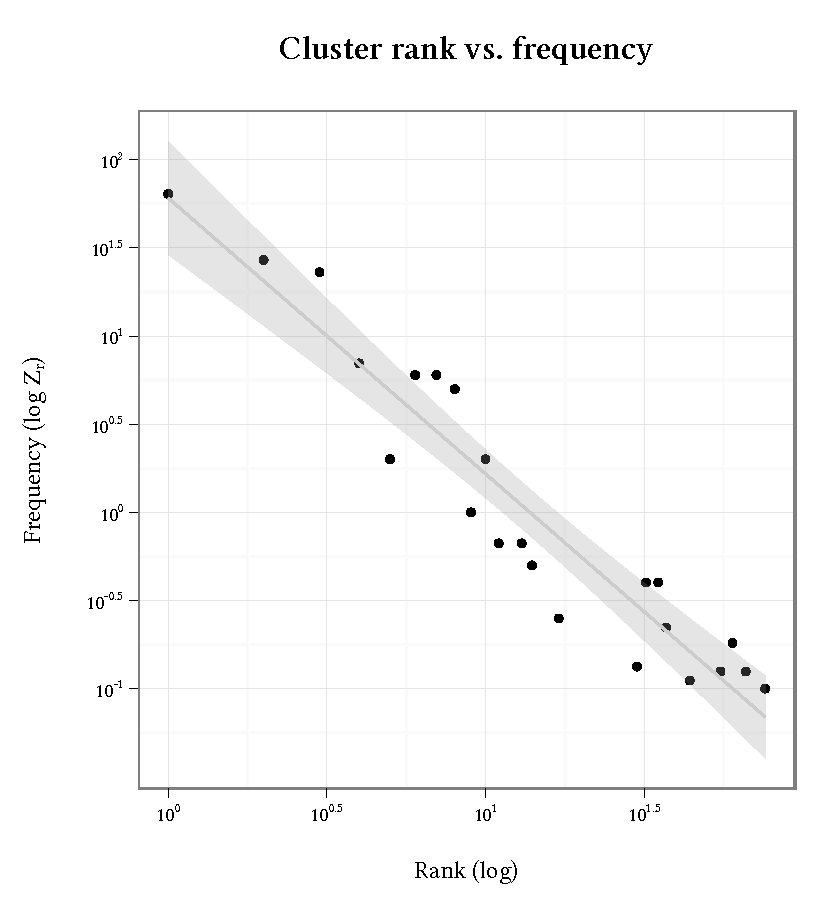
\includegraphics{cluster.pdf}
\caption{The log-log linear relationship between frequency and rank demonstrates that syllable contact clusters are Zipf distributed.}
\label{clus}
\end{figure}

It is important to note that there is nothing inherently meaningful about the fact that clusters conform to a Zipfian distribution. These distributions characterize the frequencies of many linguistic objects, from syntactic rules \citep{Yang2009} to word \citep{Teahan1998,Ha2002,Baroni2009} and phoneme \citep{Daland2011a} $n$-grams, but are also found in non-linguistic symbol systems \citep{Chomsky1958,Sproat2010} and randomly generated texts \citep{Miller1957,Li1992}. The importance of this statistical property is that it entails a long right tail, making it difficult to determine on statistical grounds alone which unobserved events are impossible and which are accidental gaps due only to the sparsity of the data. 

\subsubsection{The Good-Turing estimate}

\citet{Good1953} proposes an estimate of $\hat{p}_0$, the probability of all unseen events, originally developed in collaboration with Alan Turing. This probability is simply $n_1$, the number of events which occur just once, divided by the number of observations.

\begin{unlabeledexample}
$\displaystyle \hat{p}_0 = \frac{n_1}{\displaystyle\sum N}$ 
\end{unlabeledexample}

\noindent In CELEX, $65$ clusters occur only once, and there are 873 cluster tokens, so $\hat{p}_0 = 0.074$. The interpretation of this quantity is as follows: were possible to generate a new corpus of syllable contact clusters, approximately 7\% of the tokens would be clusters not found in the previous sample. Unfortunately, the Good-Turing estimate does not provide a way to determine which unattested clusters might be found in a replication. 

\subsubsection{Sampling simulation}

As a final consideration of this data, consider the statistical properties of a randomly generated ``lexicon'' as they compare to the observed distribution of clusters. A simulated lexicon can be generated by repeatedly applying the following procedure, which combines the derived constraint baseline with the model proposed by \citet{Pierrehumbert1994}.

\begin{example}[Simulation procedure]
\begin{tabular}{l l}
a. & Sample a medial coda according to the observed probabilities  \\
b. & Sample a medial onset according to the observed probabilities \\
c. & Apply all matching \emph{SPE} rules to the resulting clusters \\
\end{tabular}
\end{example}

While this procedure can be repeated indefinitely, it is worthwhile to consider the results of a single characteristic ``lexicon'' produced in this fashion. The slope of the log-rank/log-frequency relationship for the simulated data ($\alpha = -0.524$) is also close to the observed slope for the CELEX data ($\alpha = -0.588$). And, as shown in Figure \ref{sim}, the two distributions are nearly indistinguishable. 

\begin{figure}
\centering
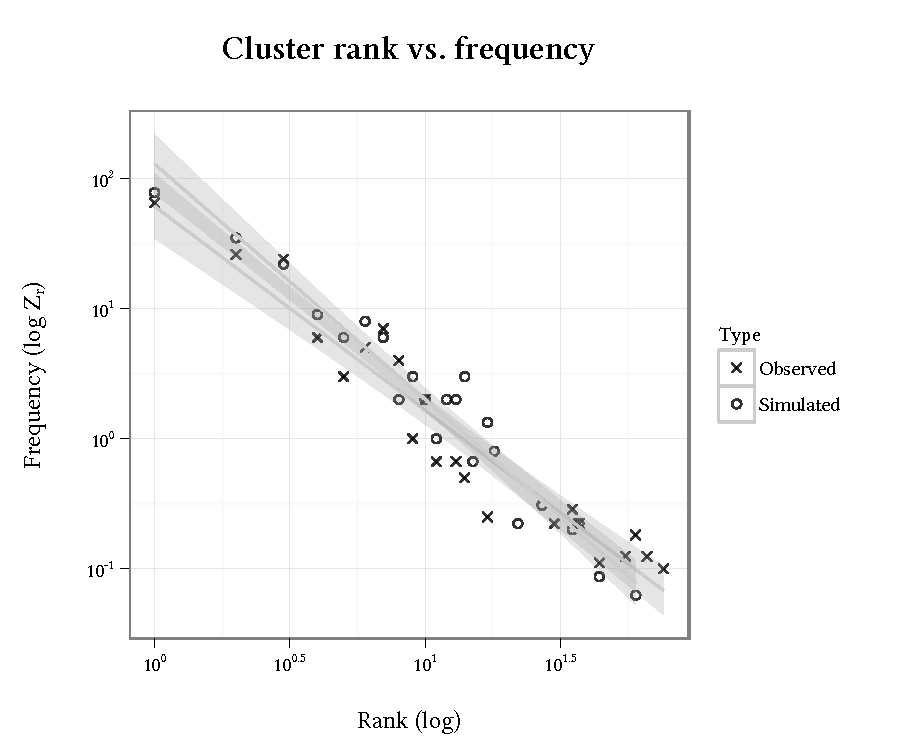
\includegraphics{sim.pdf}
\caption{The observed cluster frequencies are closely matched by a simulated cluster inventory generated by random sampling.}
\label{sim}
\end{figure}

This result should not be construed as an endorsement of the \citet{Pierrehumbert1994} model. Rather, it shows that even if the only constraints on syllable contact clusters are that they must consist of valid medial codas and onsets which further conform to the three derived constraints, there still will be many gaps in the cluster inventory, gaps which are quite arbitrary from the perspective of the phonology.

\section{Conclusion}

\citet{Borowsky1989} on peripherality.
productive \citet{Duanmu2008}

The next two chapters return to the question of synchrony, addressing the relationship between statistical patterns in the lexicon and speakers' behaviors when presented with underrepresented sequences.

accidental gaps
\citet[][419f.]{Hayes2008a}

%as in \emph{a}[b.s]\emph{inth} and \emph{a}[s.b]\emph{estos} CELEX also contains \emph{jo}[d.p]\emph{urs}, \emph{pi}[ntʃ.b]\emph{eck}, \emph{sa}[k.b]\emph{ut}, and \emph{ja}[k.d]\emph{aw}. 
%There is no duplication between constraints on sequence structure and surface forms if both are derived from the application of the phonological rule (\citealt[][401f.]{Stanley1967}, \citealt[][382]{SPE}). 
%\citet{Wright1975} taught several nonce words to a group of adolescents, and asked them to repeat the words to each other in a game of ``Telephone''. In these nonse words, nasals do not agree in \textsc{Place} with the following obstruent in these nonsense words, and \citeauthor{Wright1975} observes that after a few rounds of the game, the nonce words had been adapted to conform to \textsc{Coda Nasal Place Assimilation}.
%\begin{example}[Artificial language adaptations (\citealt{Wright1975}:394, his transcriptions)]
%\begin{tabular}{l l l l}
%a. & [gownp] & \textgreater{} & [gump]  \\
%b. & [ǰumg]  & \textgreater{} & [ǰúŋgə] \\
%c. & [ðʌŋd]  & \textgreater{} & [tɔŋg]  \\
%\end{tabular}
%\end{example}
%\noindent If this game is akin to the process of loanword adaptation, it is possible that various extragrammatical pressures are at play \citep[e.g.,][]{Halle1998b,Dupoux1999,Ussishkin2003,Peperkamp2008}. Yet, the independent evidence for a phonological process of nasal place assimilation provides the most parsiminious account of the adaptations seen in \citeauthor{Wright1975}'s study. 
%\citet{Hay2004a} demonstrates that [n.p, mθ] clusters, which are not found in English, are in fact rated better than many attested clusters.
%The same is true of the prefix \emph{com-}/\emph{con-}, as shown by the presence of assimilation in \emph{có}[ŋ.g]\emph{ress} but not in \emph{co}[n.g]\emph{réssional}. 
%(e.g., \citealt{Bakovic2005b}, \citealt{Fruehwald2011}), 

%\ex \textsc{Coda Nasal Place Assimilation} feeds \textsc{Degemination} \citep[][116]{Borowsky1986}: \\
%\begin{tabular}{l l l l}
%a. & mature    & i[m]ature    & (cf. \emph{i}[m.b]\emph{alance})   \\
%b. & numerable & i[n]umerable & (cf. \emph{i}[n.d]\emph{ependent}) \\
%\end{tabular}
%\xe
%(\citealp{Halle1985a}:105, 
%; presumably, this generalization is limited to this one place feature because  \citeauthor{Pierrehumbert1994} also adopts the assumption that the velar nasal is derived from /n/. 
%Finally, \citet{Buchwald2005} considers [j] onglides in the speech of VBR, an aphasic patient who has difficulties producing complex onsets. 
%
%\begin{example}[VBR's complex onsets (\citealp{Buchwald2005}:79--80, his transcriptions)] \label{VBR}
%\begin{tabular}{l l l}
%a. & kəræb  & `crab'  \\
%   & bəlid  & `bleed' \\
%b. & kəwin  & `queen' \\
%   & kəwoʊt & `quote' \\
%c. & kut    & `cute'  \\
%   & musɪk  & `music  \\ 
%\end{tabular}
%\end{example}
%
%\noindent VBR breaks up complex onsets with epenthesis, including those that consist of a consonant and a back onglide cluster (\ref{VBR}b). However, no epenthesis occurs between a consonant and a front onglide; rather, the glide is absent (\ref{VBR}c). The failure of the front onglide to pattern with other consonant clusters suggests once again that the glide is part of the nucleus. 
%j
%One potential problem with this account is noted by \citet{Kaye1996}, who obseres while [juː] may follow any single tautosyllabic consonant, it never follows branching onsets unless they consist of [s] and a single consonant.This is the only sign that [juː] shows an affiliation for the onset. 
%In fact, [t.ʃ, d.ʒ] clusters are not found in simplex English words, despite the fact that that affricates occur as medial onsets in clusters (e.g., \emph{tru}[n.tʃ]\emph{eon}, \emph{so}[l.dʒ]\emph{er}).
%Finally, \citet[][251]{Fromkin1973} also presents evidence that post-vocalic \emph{r} may behave as if nuclear in speech errors. 
%\citep[e.g.,][142]{Mester1988}.
%\footnote{English glides are transcribed here as full segments, not as ``subsegments'', as this distinction does not appear to be meaningful for English, or a part of a contrast in any known language \citep{Rubach2002}.}
% Note that [tʃ] has not been included since it so rarely occurs in clusters.
%\subsubsection{Summary}
%
%The above results are summarized in Table \ref{constraints}.
%
%\begin{table}
%\centering
%\begin{tabular}{l r r r r r}
%\toprule
%                                       & \multicolumn{2}{c}{attested} & \multicolumn{2}{c}{unattested} & \multirow{2}{*}{$p$-value} \\
%                                       & conforming & violating & conforming & violating \\
%\midrule
%\textsc{O.V.A.} (\ref{ovar})        &  80 &   6 & 370 & 264 & 1.1\e{-11} \\
%\textsc{C.N.P.A} (\ref{CNPA})       &  41 &  25 &  12 &  42 & 1.7\e{-05} \\ 
%\textsc{Degemination} (\ref{degem}) & 161 & 632 &   0 &  87 & 1.4\e{-08} \\
%\midrule
%\textsc{*Dorsal-Labial} ()          &  68 &   4 & 246 &  40 & 0.069 \\
%\textsc{*C.C.O.} ()                 &  48 &  38 & 312 & 322 & 0.301 \\
%\textsc{*A,BA} ()                   & 161 &   0 & 708 &  11 & 0.231 \\
%\bottomrule
%\end{tabular}
%\caption{Counts and Fisher exact test $p$-values for the constraints discussed above.}
%\label{constraints}
%\end{table}
%Whereas 18.8.\% of the ``possible'' clusters are attested, 28.8\% of those which conform to these three constraints are found. 
%Binary classification contingency table: \\
%\begin{tabular}{c | l l} \toprule
%                             & \multicolumn{2}{c}{prediction} \\
%\midrule
%\multirow{2}{*}{observation} & true positive ($tp$)  & false positive ($fp$) \\
%                             & false negative ($fn$) & true negative ($tn$) \\
%\end{tabular}
%\begin{tabular}{|l l|}
%\toprule
%true positive ($tp$)  & false positive ($fp$) \\
%false negative ($fn$) & true negative ($tn$) \\
%\bottomrule
%\end{tabular}
%\begin{figure}
%\centering
%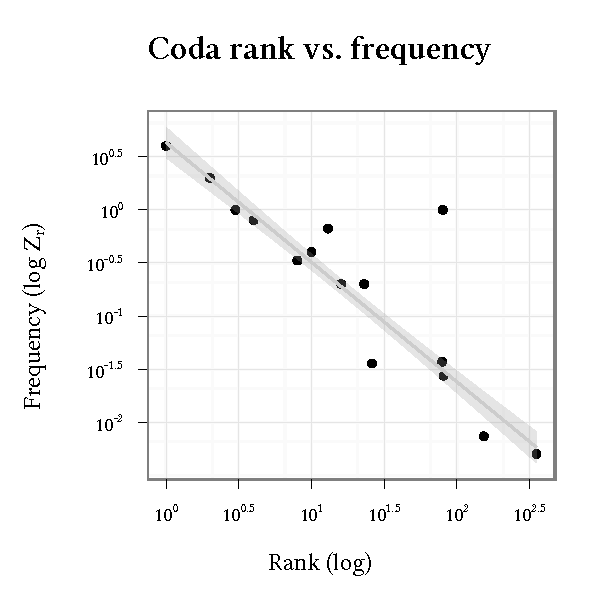
\includegraphics{coda.pdf} 
%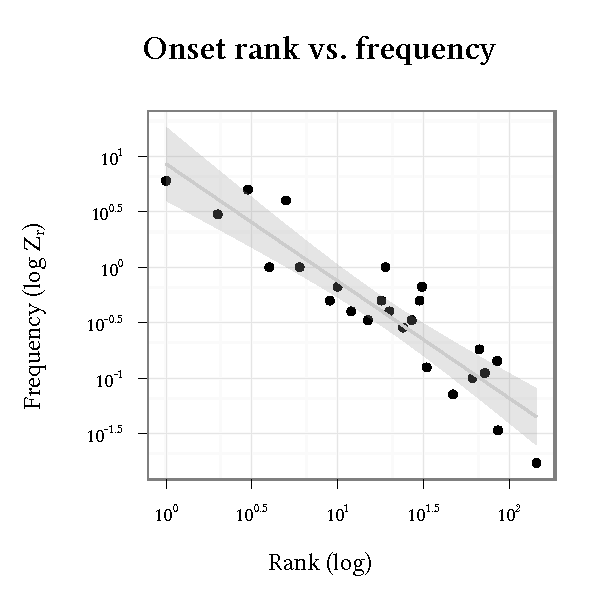
\includegraphics{onset.pdf}
%\caption{Medial coda and medial onset lexical frequency exhibit the Zipfian log-log-linear relationship between rank and frequency.}
%\label{codaonset}
%\end{figure}
%Sparsity alone is not the only reason for cluster underrepresentation which is external to the phonology. For instance, a cluster could be underrepresented due to language change. \citet{Iverson2005} discuss a case of this type: In English, long vowels before word-final [ʃ] in English are generally rare (though note ``affective'' \emph{swoosh}, \emph{sheesh}, etc.). This is ultimately due to the fact that native [ʃ] is descended from Old English [sk], and long vowels are not fonud not occur before complex codas. \citeauthor{Iverson2005} conclude that this gap is accidental because it does not inhibit borrowing and coinage. 
%On the other hand, patterns created by sound change are not guaranteed to persist over time. One example of non-persistence is discussed by \citet{Iverson2005}. Around 1100 CE, Old English \emph{sk} became [ʃ]. This sound change introduced no alternations. Since long vowels were not found before tautosyllabic syllable clusters at this time, there were no \emph{V\lm sk\#} words when the change was actuated, and \emph{V\lm sh\#} continues to be rare in Modern English. What \citeauthor{Iverson2005} observe, however, is that there is nothing apparently peripheral about words like \emph{leash} or \emph{whoosh}, and loanwords and coinages have readily filled the gap.
%\citet[][140]{Frisch2004} suggest that the strong tendency for the first and second consonants of the Arabic root to be non-identical is the ``a diachronic result of a processing constraint that disfavors repetition.'' Unfortunately, there is no evidence that this pattern is diachronic other than in the sense that it appears to be inherited from the proto-language: there is simply no Proto-Semitic verb roots with identical first and second consonants \citep[][178]{Greenberg1950}. In other Semitic languages, the inherited patern has experienced considerable erosion. 
%
%\begin{example}[Tigrinya roots with identical first and second consonants \citep{Buckley1990a}]
%\begin{tabular}{l l l l}
%a. & lʌlʌw     & `scorch'                   & (\textless{} Ge'ez \emph{lʌwlʌw} `inflame')     \\
%   & mʌmʌy     & `winnow'                   & (\textless{} Ge'ez \emph{mʌymʌy} `distinguish') \\
%   & mʌmʌt     & `pick out loot'            \\
%b. & s’ʌs’ʌw   & `finish off a drink'       & (cf. \emph{s’ʌws’ʌw} `gulp down')           \\
%   & t’ʌt’ʌf   & `prune tree'               & (cf. \emph{t’ʌft’ʌf} `smear wall with mud') \\
%c. & kʷakʷkʷʌr & `waste away, be emaciated' & (cf. \emph{kʷarkʷʌr} `interrogate')         \\
%   & kakʷkʷɨʕ  & `clean wax from ears'      & (cf. \emph{kaʕkʷɨʕ} `start to form pods')   \\
%\end{tabular}
%\end{example}

%Similar exceptions are found in 
%Amharic (\citealp[][?]{Broselow1984}, \citealp[][?]{McCarthy1985}) and 
%Hebrew \citep[][29]{Bat-El2005}.
